%location/filename: tex/ch1.tex
%author: Anders Østevik
% Created: 28.2.2016
%#######--Chapter 4--#######
%Content:	

\documentclass[main.tex]{subfiles}

%\usetikzlibrary{arrows,automata}

\begin{document}

\chapter{Loopback Test using the GBT Quartus Example}

\section{GBT Quartus Example}


\section{120 MHz Reference Clock}

%\todo{name the proper plls and state why 120 mhz is really needed} 

To be able to conduct a proper loopback test, the \gls{mgt} and the \glspl{pll} of the \gls{gbt} example design must have a input clock frequency of $120~\mega\hertz$. There are a number of ways to achieve this on the Cyclone V board: 
\begin{itemize}\setlength{\itemsep}{10pt}
\item Using an external clock, like a square wave signal generator.
\item Using one of the onboard programmable oscillators.
\item Implementing a \gls{pll} into the design that multiplies the onboard $50~\mega\hertz$ global clock up to the desired frequency of $120~\mega\hertz$.\\
\end{itemize}

The original approach is to use an external signal generator with differential output to generate the reference clock, as shown in the \gls{gbt} tutorial videos \cite{gbt_videos}. However, at the time of conducting the first tests, there was no available signal generators that could generate a $120~\mega\hertz$ square wave clock for the experiment. Because of this, some time was spent to investigate how to use the internal programmable oscillator as a reference clock.

The approach of implementing an extra \gls{pll} into the \gls{gbt}-example design was also investigated, but attempts of doing so resulted in conflicts between the already implemented transceiver \glspl{pll} in the design. \\

The below sections gives the following descriptions:
\begin{itemize}\setlength{\itemsep}{10pt}
\item How to setup the onboard oscillator on the Cyclone V GT board for use as reference clock (\ref{sec:inclk}). 
\item How to setup the $Si5338$ external oscillator for use as reference clock (\ref{sec:exclk}).
\end{itemize}

\subsection{Configuring the onboard Oscillator on the Cyclone V Board} \label{sec:inclk}

To achieve a reference clock of $120~\mega\hertz$ without an external clock, the \gls{fpga} has an onboard programmable oscillator; the $Si570$ from Silabs. It uses \gls{iic} for serial communication and can be programmed to output frequencies up to $810~\mega\hertz \pm 50 ppm$. To program the oscillator, Altera provides a dedicated software called "Clock Control". The Clock Control software is part of the Java based "Board Test System" software, included in the Cyclone V kit which can be found at Altera's websites \cite{altera_cyclonekit}. The Cyclone V kit is board specific, so it is therefore important to use the right kit with the right board.\\

To make use of the Clock Control software has been proven difficult, mainly because of the software being outdated in relevance to the current version of Quartus (at the time of writing, Quartus 15.0 is the newest edition). The solution was to install an older Quartus (version 13.1) using the Windows Operating System (Linux was also attempted, but without any success) and specify the right paths for the related environment variables. See appendix \ref{chap:clksetup} for a description on how to setup the clock control software using Windows.

\subsection{Configuring the Si5338 External Oscillator} \label{sec:exclk}

For an external clock, the $Si5338$ evaluation board was used (figure \ref{fig:si5338}). It has an onboard $25~\mega\hertz$ XTAL oscillator in addition to six SMA connectors reserved for external input clocks. For simplicity, the onboard oscillator was used in the thesis experiments. The remaining eight SMA connectors is reserved for differential output clocks. The evaluation board communicates with \gls{iic} and connects to the \gls{pc} via \gls{usb} cabling. A dedicated clock builder software \cite{siclk} lets you select clock outputs and type of signaling. For the experiments, a $2.5~\volt$ \gls{lvds} clock with $120~\mega\hertz$ was selected, and connected to the Cyclone V GT board using SMA cabling. To enable the SMA connectors as input to the reference clock on the Cyclone V GT board, \textit{CLKSEL} on DIP switch SW4 must be selected ON (default is OFF).

\begin{figure} % H(strictly put HERE > h!)
\begin{center}
% h(here), !(force), t(top), b(bottom), p(on extra page)
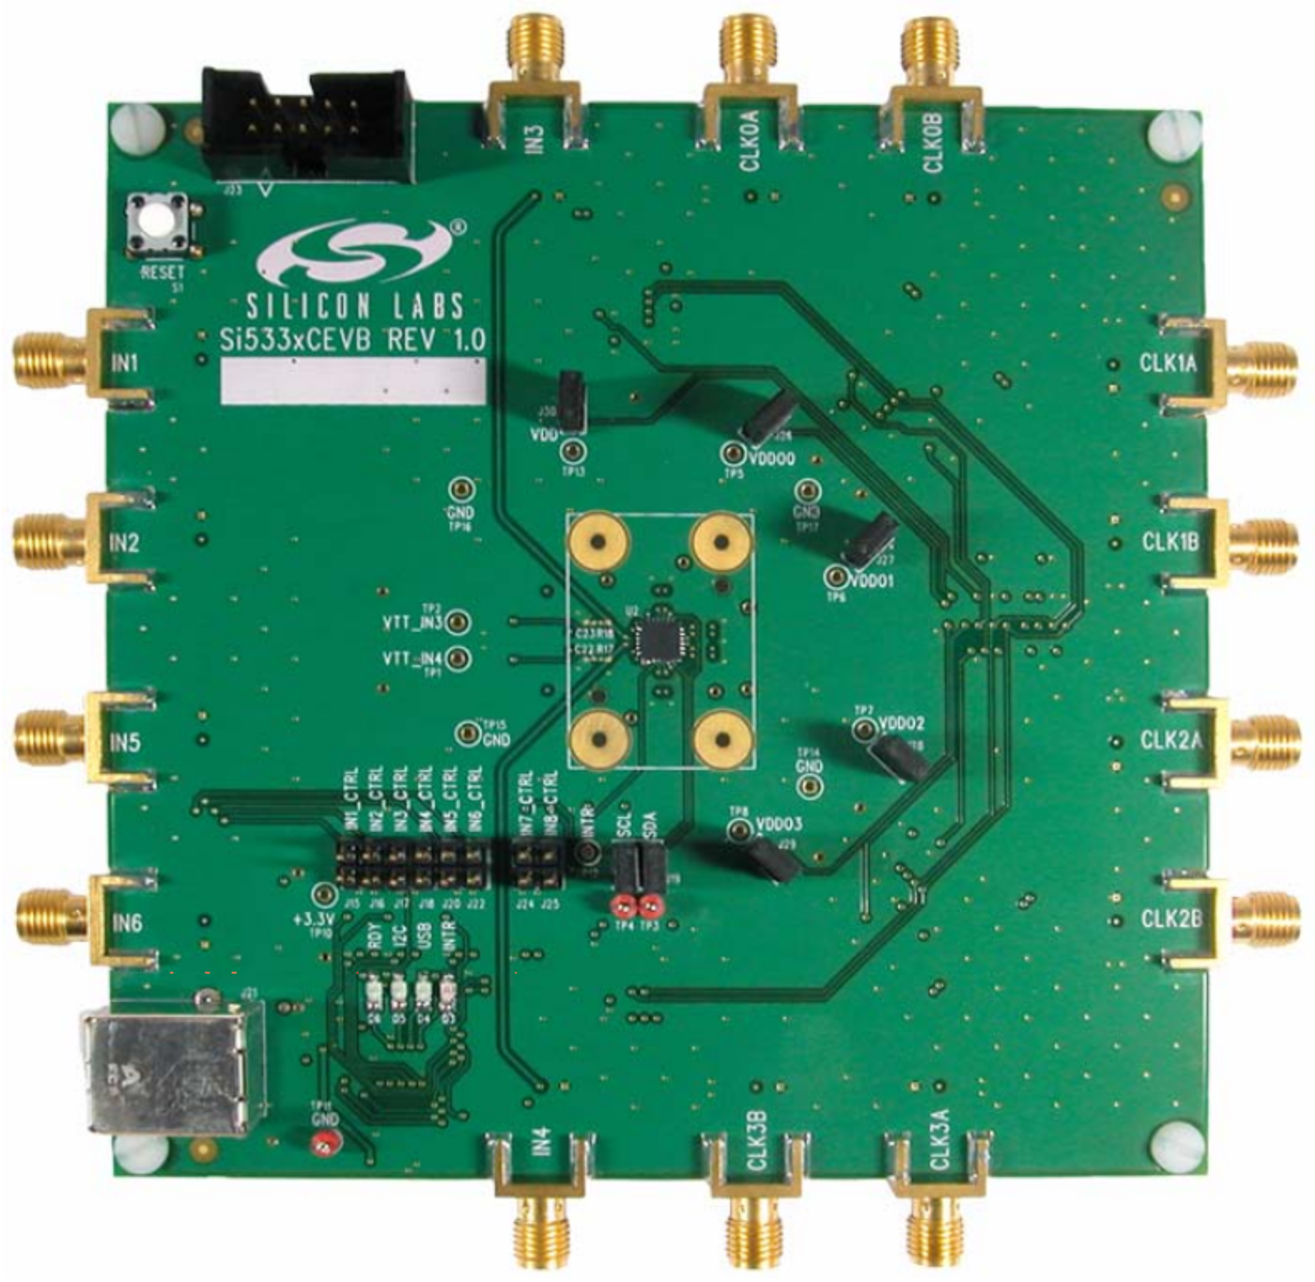
\includegraphics[scale=0.3]{../img/si5338}  \\[0.1 cm]
\caption{The $Si5338$ evaluation board \cite{si16}.}
\label{fig:si5338}
\end{center}
\end{figure} 

\section{Testing and Verification of the HDMI Daughter Card}
To verify a working \gls{pcb}, the \gls{hdmi} daughter card underwent a series of tests. The sections below summarizes these tests. 

\subsection{Connectivity Test}

\textit{Since all the components on the \gls{pcb} was hand soldered (with the exception of the ground pads underneath the \gls{hsmc} contact), it was particularly important to check for accidental shorts between pins and/or pads.}

\subsubsection{Purpose of Test}

\begin{itemize}\setlength{\itemsep}{10pt}
\item Verify that there are no shorts between the pins and/or pads of the \gls{pcb}. 
\item Check for current draw to confirm that there are no short on the power-lines.
\end{itemize}

\subsubsection{Experimental Setup}

The setup involves the use of a multimeter to go through all pins and check for connection faults according to the schematic. After all shorts have been eliminated, the \gls{pcb} is to be connected to an external power supply to verify current-draw. 

\subsubsection{Results}
 Using a multimeter, all connections were checked and verified that there were no shorts (Some pins on the \gls{hsmc} were indeed shorted and had to be re-soldered). The \gls{pcb} was then connected to an external power supply, with a $3.3~\volt$ output and a current output limited to $100~\milli\ampere$. It was verified that the current draw, with all \gls{hdmi}-connections left open, were no more than the current drawn from the power-\acrshort{led} and the $1.25~\volt$ voltage divider, i.e around $40~\milli\ampere$. \\

To confirm connectivity and that there were no further connecting shorts between the pads and/or pins, a simple test-circuit was written in Quartus. Beginning with the transmit-signals: all the relevant \gls{lvds} transmit-signals that are physically connected to the \gls{hsmc} (port A) connector of the \gls{fpga} were connected to a given clock signal. The \gls{pcb} was then connected to the Cyclone V board, and the \gls{hdmi} connectors were probed with the help of an oscilloscope and verified that there was an output signal on every \gls{hdmi}-transmitter. 

The \gls{pcb} is now ready for connection with the host \gls{fpga} for further testing of the transmitter and receiver signals. 

\subsection{External Loop-back Test for the Fiber-Optic Connector} \label{sec:exlooptest}

\textit{To verify that the \gls{hdmi} daughter card SFP-connector for fiber-optic communication is working correctly, an external loop-back test was conducted.}

\subsubsection{Purpose of Test}
\begin{itemize}\setlength{\itemsep}{10pt}

\item Test the dedicated SFP-connector on the \gls{hdmi}-daughter card for fiber-optic communication and see that it is capable of sending and receiving information at speeds corresponding the \gls{gbt}-standard of $4.8 \giga\bit\per\second$. 
\end{itemize}

\subsubsection{Experimental Setup}
A fiber-optic cable connected from the transmitter to the receiver using a fiber-module, forming an external loop through the cable, was connected to the SFP-connector of the \gls{hdmi}-daughter card \gls{pcb}. Using the \gls{gbt} Quartus-example together with the \gls{issp} and SignalTap II, it was possible to perform a pattern check test by comparing the transmitted signals with the received signals. To achieve this test, \gls{issp} was used to setup the pattern generator of the GBT example to count with increments of one (PATTERN SELECT = "1h") and the receiver to receive signals through external cabling (LOOPBACK = '0'). SignalTap II was used to monitor and verify that the receiver line received the same incremented counter that the transmitter sent out.

\subsubsection{Results}
Running the test resulted in a continuous stream of bits sent from the transmitter to the receiver. Using SignalTap II as a monitor limits to only observe parts of the transmission, but it was sufficient enough to see that the received sum of bits were indeed incrementing by one each time. The results are comparable with the same test using internal loopback (LOOPBACK = '1'), i.e observing that the receiving end is counting by increments of one. This concludes that the SFP-connector on the HDMI-daughter card works as intended at the desired speed of $4.8 \giga\bit\per\second$. Figure \ref{fig:lb_rx} shows the resulting incremented sum of bits transmitted and received at the receiving end.


\subsection{External Loop-back Test for the HDMI Connectors}

\subsubsection{Purpose of Tests}

\begin{itemize}\setlength{\itemsep}{10pt}
\item Measure the quality of the signal (eye-diagram) at different frequencies up to $300~\mega\hertz$ and see how reflections affects the signal.
\item Measure crosstalk between neighboring signal paths.
\item Create a test environment using Quartus II in conjunction with SignalTap II to:
\begin{itemize}\setlength{\itemsep}{10pt}
  \item See if it is possible to sample the received signals at different frequencies up to $300~\mega\hertz$.
  \item Calculate the bit-error rate at different frequencies up to $300~\mega\hertz$.
\end{itemize}
\end{itemize}

\subsubsection{Experimental Setup}

Each \gls{hdmi}-connector has at least one transmitter- and receiver line. To simulate signal transmission over a distance, a \gls{hdmi} cable was cut in half and the transmit- and receive lines were soldered together, creating an external loop-back. VHDL code was written to simulate a data-stream using a pseudo-random generator to generate random bit-patterns. The data-stream would travel out via one of the transmitters of the \gls{fpga}, out through the \gls{hdmi}-connector, following the cable back into the same \gls{hdmi}-connector into the receiver input. This would simulate the transmission path to the \gls{vldb} card. The transmitted and received bits would then be compared using xor-logic. A bit-counter register would count each transmitted bit, and a bit-error register would count each time two bits are different in comparison. The bit error rate is thus given by $\frac{bit~errors}{number~of~bits}$.

Because of the trace- and cable-lengths and the fact that a signal has a finite propagation time, a delay is introduced between the transmitted and received bit-signals.\footnote{As mentioned in chapter \ref{chap:pcb}, a signal propagates through the conductor at a velocity of approximately $15\ \milli\meter/\nano\second$.} To cope with the delay differences, a delay chain is added in parallel with the transceiver line: While a bit-signal is travelling through the cable, the same bit-signal is delayed through a series of \glspl{dff}. For each clock cycle, the value at the receiver input is compared with the output of each \gls{dff} using XOR-logic. The individual outputs of the XORs are connected to \glspl{led}. The \gls{led} that has the least amount of toggling is the one XOR, and thus selected \glspl{dff}, that is most synchronized with the receiver (ideally, it should be toggle-free), and can be used to count bit errors. A smaller delay-chain was also added at the receiver line to synchronize the incoming bits with the clock. Figure \ref{fig:delaych} a and b illustrates these delay chains.

\begin{figure}
    \centering
    \begin{subfigure}{\textwidth}
        \centering
        \resizebox{1\linewidth}{!}{\subfile{fig_txdelay.tex}}
        \caption{Delay chain on the transmitter line.}
    \end{subfigure}

    \begin{subfigure}{0.6\textwidth}
        \centering
        \resizebox{1\linewidth}{!}{\subfile{fig_rxdelay_0.tex}}
        \caption{Delay chain on the receiver line.}
    \end{subfigure}
    \caption{Transmitter and receiver delay chains.}
    \label{fig:delaych}
\end{figure}

Cables with different lengths were used to see how this would affect the bit-error rate. This would thus introduce varying delay differences between the transmitter and receiver, and would therefore produce different results comparing the signals in the delay chain. A series of attempts were therefore made to find the most synchronized outputs of the delay-chains at different cable lengths. 

%To measure the quality of the \gls{lvds} signals with an oscilloscope, differential probes were used.  

\subsubsection{Results}

%The following table sums up the cable-length and theoretical travel time versus the measured delay between the transmitted and received signal.

During the first samplings using SignalTap II, it was suspected that when running at a $300~\mega\hertz$ clock, the received signal were being sampled when in a metastable state, i.e in the middle of the rising edge of the bit. To compensate for this, a new delay chain was designed on the receiver line (figure \ref{fig:rxpardelay}): two \glspl{dff} that would trigger on different clock edges (rising and falling), were placed in parallel as the first stage of the receiver delay chain. By using a MUX, one of the \gls{dff} outputs were selected to go into a third \gls{dff}, and the output of this third \gls{dff} was then compared with all outputs in the transmitter delay chain. The "Rising/Falling DFF" tab in table \ref{tab:delch} states which of the clock edges that caused less toggling the first delay stage on the receiver. When sampling the \glspl{led} using SignalTap II, some "spikes" occurred at the \gls{led} that seemed toggle-free when observing it. The "spikes" were narrower than the $300~\mega\hertz$ clock, and seemed to occur randomly. Whether this will affect the error-counter hasn't been confirmed, as the test was aborted due to an accident with the \gls{fpga}. The accident caused two of the pins on one of the current regulators on the FPGA board to short, resulting in a burned regulator. This rendered the FPGA useless and halted all remaining tests. Due to time constraints, the \gls{fpga} was not repaired in time for the delivery of the thesis.  

%With this new delay chain design, it seemed that using only \glspl{dff} with rising edge clock triggering worked the best. Some "spikes" were detected on the XOR-output with SignalTap II. These spikes were much narrower than the clock signal. What caused this might 

\begin{figure}
    \centering
    \resizebox{0.7\linewidth}{!}{\subfile{fig_rxdelay.tex}}
    \caption{Muxed delay chain on the receiver line.}
     \label{fig:rxpardelay}
\end{figure}

With the help of SignalTap II it was possible to sample the delay chain signals and produce the results displayed in table \ref{tab:delch}. 
\begin{table}
\centering
\caption{SignalTap II measurements on the J10 hdmi connector of the HDMI daughter card. "sync\#"" is the most synchronized XOR-output in the delay chain. Length is the approximate traveling path (cable and trace) for the signal. The "Rising/Falling DFF" tab shows which edge triggered DFF that worked best as the first stage at the receiver delay chain.}
\label{tab:delch}
\begin{tabular}{|p{1cm}|p{1.5cm}|p{2cm}|p{2.5cm}|p{5cm}|}
\hline
 Clock [Mhz]  & sync\#   & Signal path [cm]   & Rising/Falling DFF  & Comments \\ \hline
 100          & 1     & 110           & Rising              & Some spikes occur.  \\ \hline
 200          & 2     & 110           & Rising              & No spikes. \\ \hline
 300          & 4     & 110           & Both                & No spikes. \\ \hline
 %\multicolumn{5}{|l|}{} \\ \hline
 100          & 1     & 220           & Rising              & Some spikes occur.\\ \hline
 200          & 3     & 220           & Rising              & Some periodical spikes.\\ \hline
 300          & 5     & 220           & Rising              & No spikes.\\ \hline
\end{tabular}
\end{table}

Unfortunately, while doing the above test, an accident caused two of the pins on one of the current regulators on the FPGA board to short, resulting in a burned regulator. This rendered the FPGA useless and halted all remaining tests and 

\subsection{Conclusion and Discussions}

When measuring a high-speed signal, the way you measure the signal can have a major impact on the result. This was experienced when attempting to measure the \gls{lvds} signals using the differential probes. On the first attempt, small clamps connected to each of the differential probes (figure \ref{fig:hektere}) were coupled to a differential pair that were running from one end of a hdmi-cable, with a terminating resistor in between; in to a transmitter on the \gls{hdmi}-daughter card. A clock signal was sent from the \gls{fpga} throught the \gls{hdmi}-daughter card to the end of the hdmi-cable. 

\begin{figure}
   \begin{center}
     \ffigbox{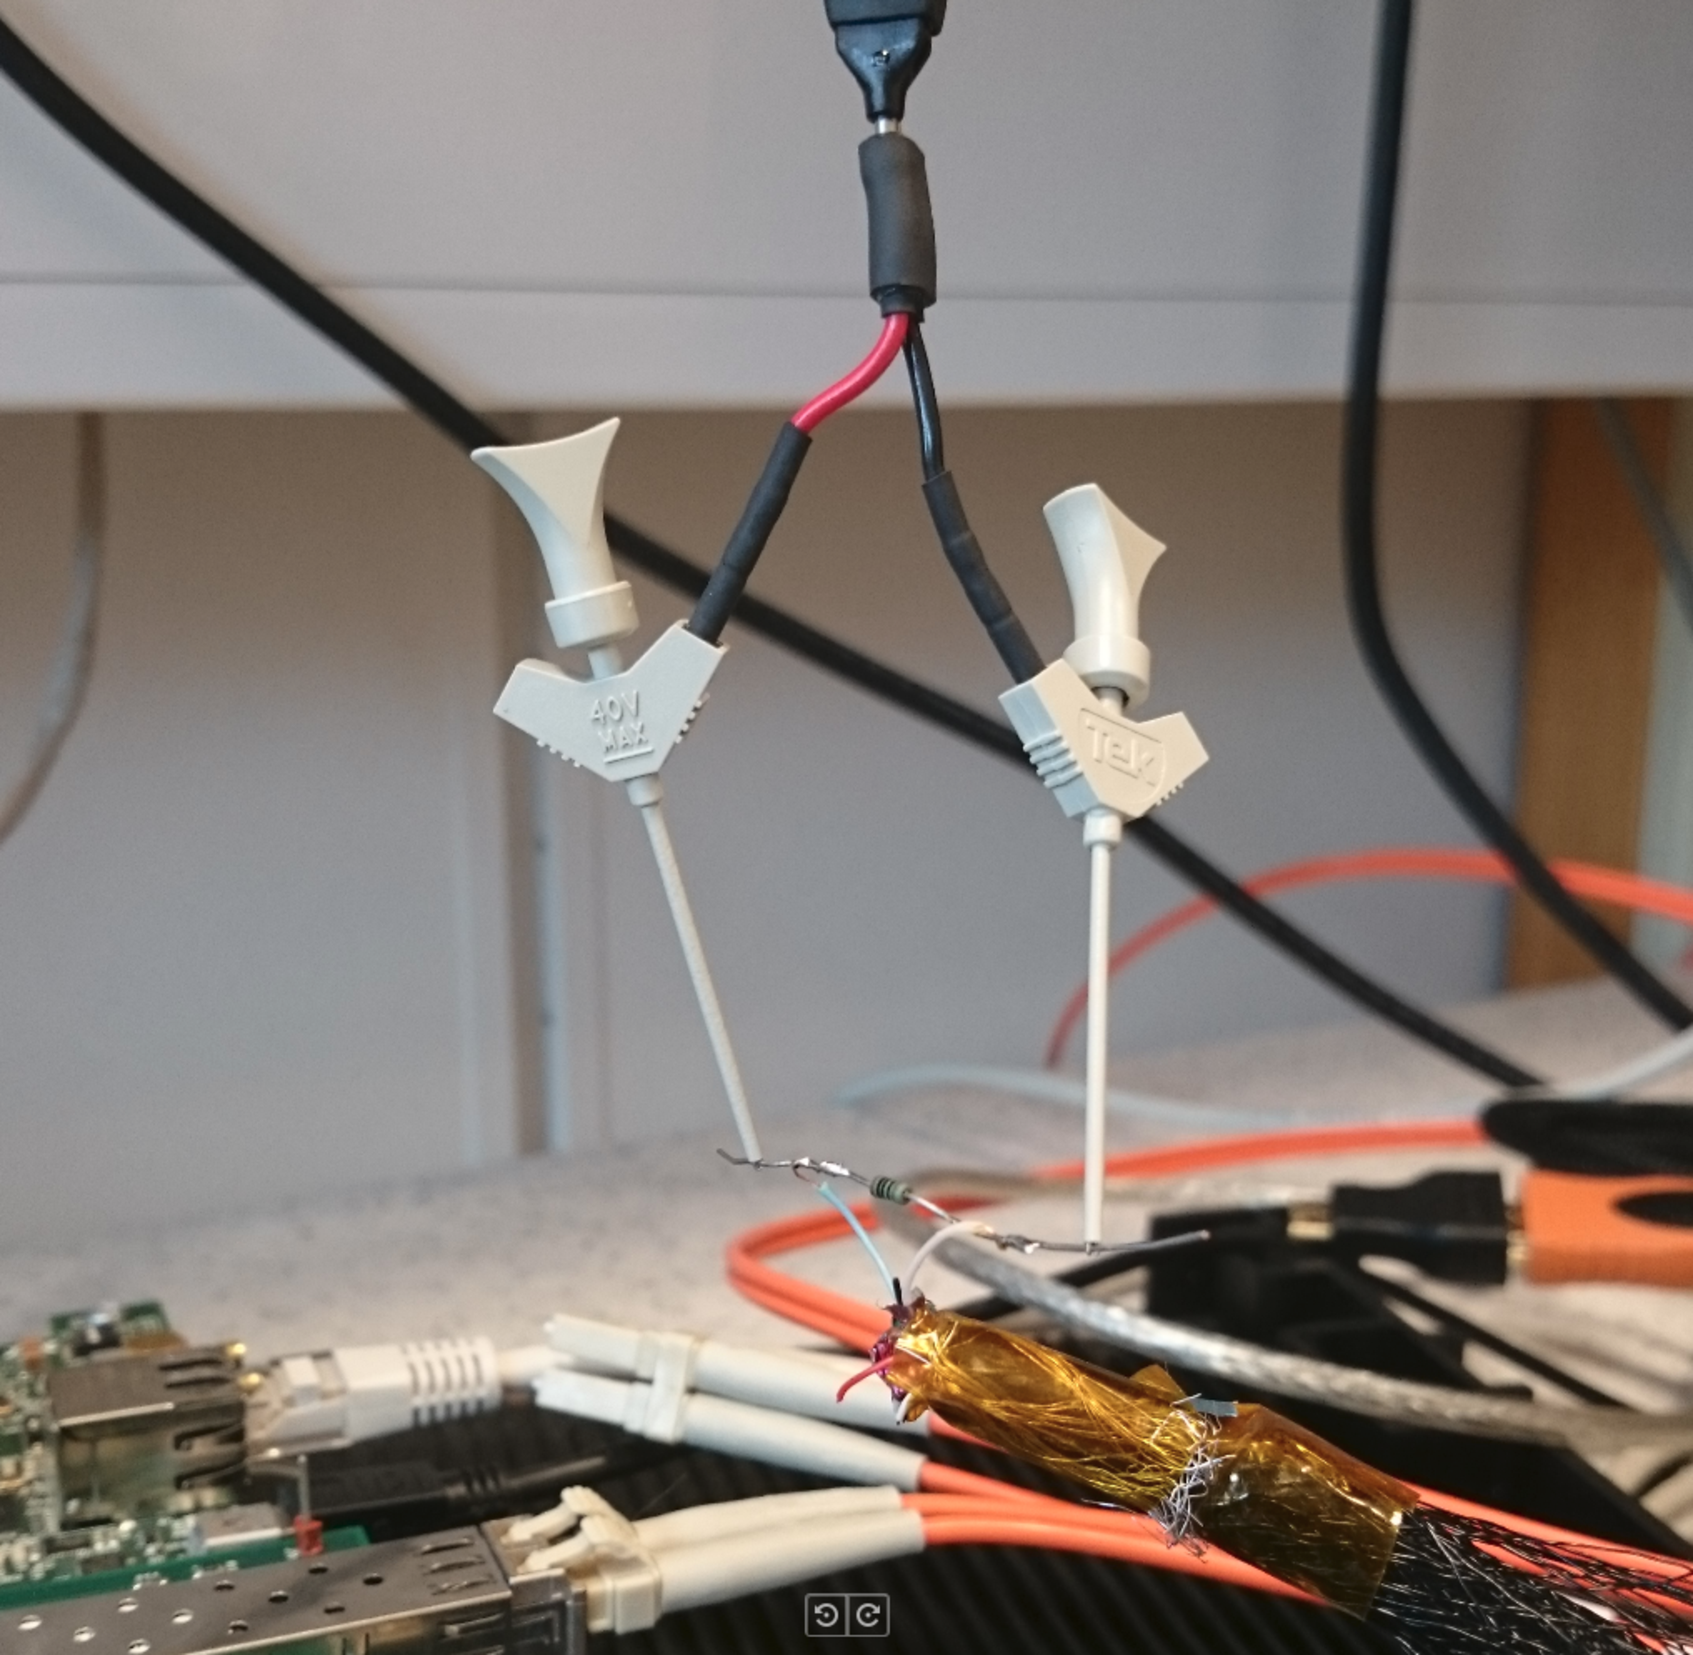
\includegraphics[scale = 0.2]{../img/hektere_probes.pdf}}{\caption{Small clamps was first used to measure the high-speed signal.}\label{fig:hektere}}
   \end{center}
\end{figure}

The measurement resulted in signals that were heavily distorted by reflections. It was first thought that these reflections might originate from the traces on the \gls{fpga} itself, since the same results were produced when sending the clock signals through a different \gls{pcb} (a GPIO-card) in place of the \gls{hdmi}-daughter card. However, the theory was quickly rejected when using a completely different \gls{fpga} board produced the same reflections. The cause was in fact due to the small clamps that was used to connect the differential probes. By replacing these with small stubs and redo the measure, the result was quite different, as shown in figure \ref{fig:measdiff}.

\begin{figure}
    \centering
    \begin{subfigure}{0.5\textwidth}
        \centering
        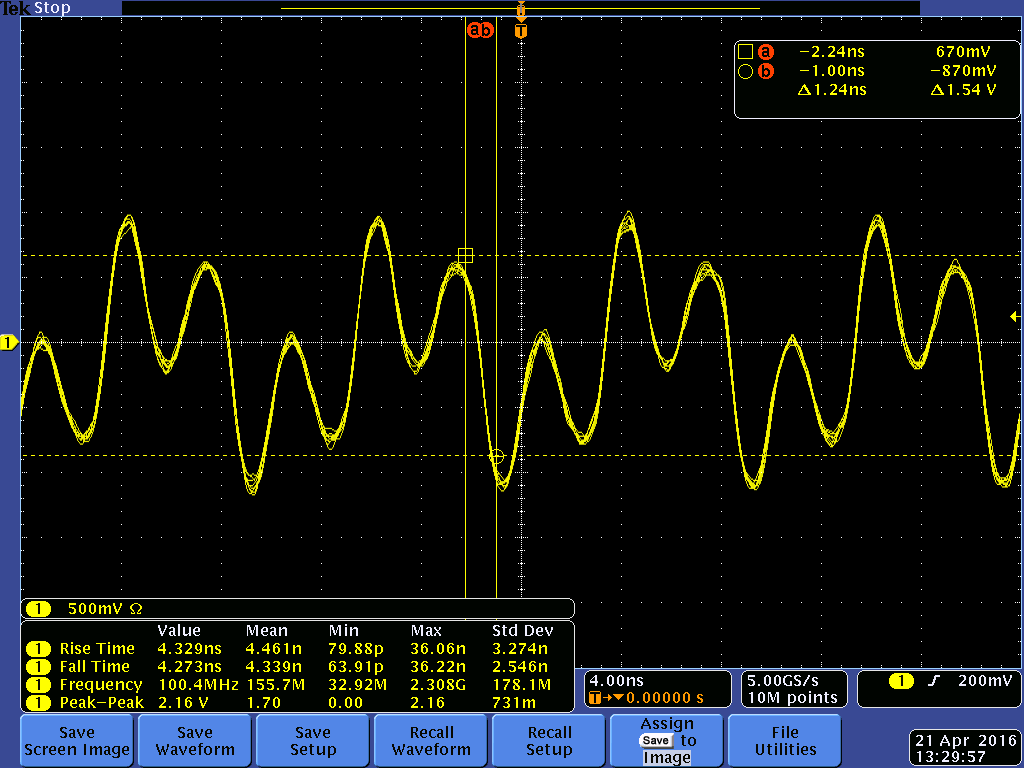
\includegraphics[width=\linewidth]{../img/hektere_oppsett_100mhz.png}
        \caption{Using clamps.}
    \end{subfigure}%
    ~~
    \begin{subfigure}{0.5\textwidth}
        \centering
        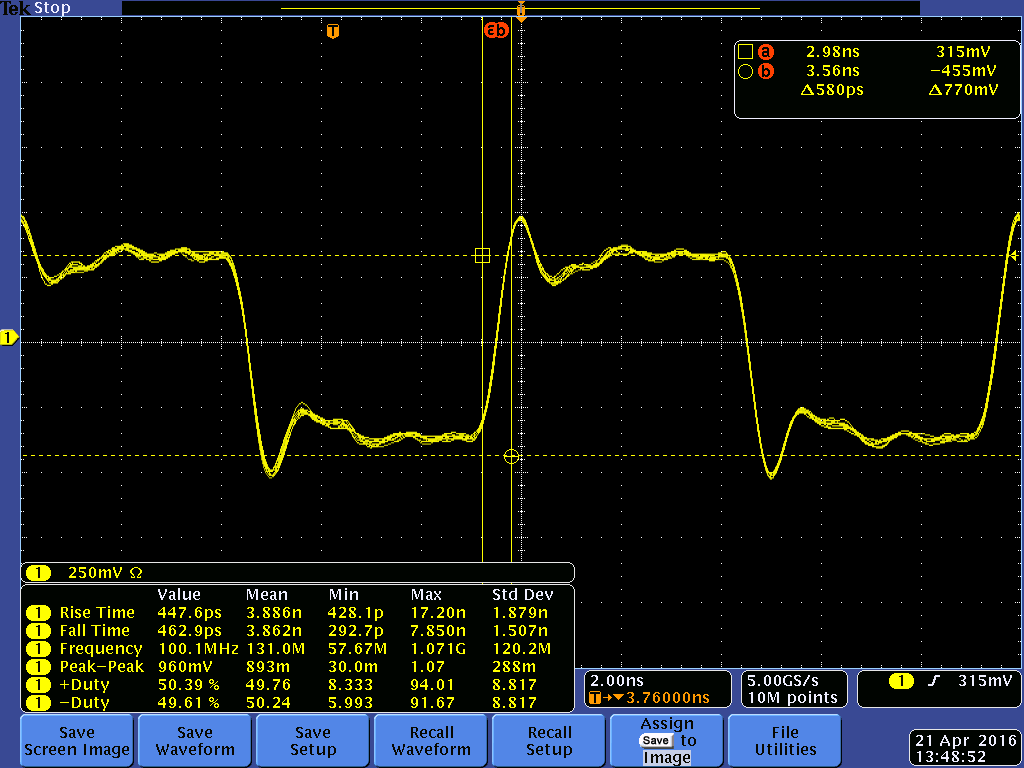
\includegraphics[width=\linewidth]{../img/stubs_oppsett_100mhz.png}
        \caption{Using stubs.}
    \end{subfigure}
    \caption{$100~\mega\hertz$ transmitter signal measured with differential probes.}
    \label{fig:measdiff}
\end{figure}

By doing the same measurements again with both the GPIO-card and the \gls{hdmi}-daughter card on both available \glspl{fpga}, the reflections remained somewhat the same. It is concluded that the most notable signal reflections is caused by the measurement setup, and will not affect the digital data when transmitting or receiving signals. This lead to the loop-back test using SignalTap II in an attempt to sample the signals (see chapter \ref{chap:sertest}).

\section{Testing and Verification of the Serial Interface} \label{chap:sertest}

\subsection{Hardware Simulation using Testbench in Modelsim}

\textit{To verify that the hardware design was working properly in terms of correct signal timing between the baudrate, \acrshort{uart} and decoder, a testbench was developed. The testbench was made using the \textit{Bitvis Utility Library} and the design simulation was done using Altera's Modelsim.}

\subsubsection{Purpose of Tests}

\begin{itemize}\setlength{\itemsep}{10pt}
\item Verify correct timing between the baudrate generator, clock and uart.
\item Verify correct timing for the uart decoder.
\item Verify that the design is working correctly in simulation.
\end{itemize}

\subsubsection{Bitvis Utility Library}
The \textit{Bitvis Utility Library} by Bitvis is an open source VHDL testbench infrastructure library for verification of FPGAs and ASICs \cite{bitvis16}. It was developed with the aim of simplifying the testbench development process when testing \acrshort{vhdl} designs. It was chosen for this test because of the ease of use and fast implementation (see uart\_tb.vhd for testbench implementation).\\

\subsubsection{Experimental Setup}
The main testbench process goes as follows: Send a request byte to the rx-signal, followed by a register-address. The request can be a read-request (0xDD) or a write-request (0xEE for '1' and 0xFF for '0'), and the address must be between 0x00 - 0xC1. Then, the tx-signal are sampled and compared with the requested address byte and checked for equality. If it is not equal, the test goes to a halt with a corresponding fault-message. The \textit{UART\_WRITE\_BYTE} and \textit{UART\_READ\_BYTE} testbench procedures were written with this in mind. To simulate an incoming byte at the receiver, \textit{UART\_WRITE\_BYTE} inputs a vector of 8 bits as the data-byte. With the period of a transmitted bit, which is equal to $1/baud rate$, it outputs first a start bit, then the data bits and finally the stop bit. The rx-line takes the output of \textit{UART\_WRITE\_BYTE} as input. \textit{UART\_READ\_BYTE} takes the tx-line as input, and with the period of a transmitted bit shifts the tx-value into a data vector. Using the Bitvis \textit{check\_value}-function, the data vector is then checked and compared with the address-byte previously sent to the receiver. The \textit{UART\_READ\_BYTE} procedure must be executed after the \textit{UART\_WRITE\_BYTE} procedure. \\

Other test procedures involves checking the constants found in \textit{uart\_gbt\_pkg.vhd} up against legal values, and also make sure that the tx- and rx-lines are in an idle state at the start of the test, i.e a high state.

\subsubsection{Results}

Figure \ref{fig:uarttb} shows three read operations followed by a write operation. The $tx\_data\_compare$ vector compares the address received with the address transmitted to confirm that the \gls{uart} decoder does what it is requested to, i.e send out the correct addresses when receiving a read-request and write a bit-value to the \gls{gbt} register when receiving a write-operation. The data-bit (\gls{msb} of the transmitted signal) is not included in the $tx\_data\_compare$ comparison, nor is the write operation. 

\begin{figure}
    \centering
    \begin{subfigure}{0.18\textwidth}
        \centering
        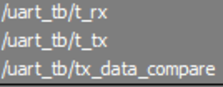
\includegraphics[width=\linewidth]{../img/uart_tb_0}
    \end{subfigure}%
    \begin{subfigure}{0.7\textwidth}
        \centering
        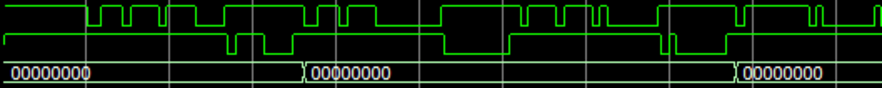
\includegraphics[width=\linewidth]{../img/uart_tb_1}
    \end{subfigure}
    \caption{Three read operations followed by a write. }
    \label{fig:uarttb}
\end{figure}

\subsection{Running the PC software design together with the FPGA hardware design} \label{test:designrun}

\textit{Check if the \gls{fpga} design is responding correctly to the bytes sent from the C-program on the \gls{pc} side.} 

\subsubsection{Purpose of Tests}
\begin{itemize}\setlength{\itemsep}{10pt}
\item Verify that the C-program is in control of the COM port.
\item Verify that there is communication between the \gls{fpga} \gls{uart} and the \gls{pc} COM port.
\item Confirm that the \gls{fpga} design and C-program is working together the way they should.
\end{itemize}

\subsubsection{Experimental Setup}

The Cyclone V Gt \gls{fpga} was programmed with the hardware design (\ref{chap:hardware}) and connected to the user PC using a USB-to-RS232 cable with a $5~\volt$ voltage converter between the FPGA and the cable. The software was granted PC admin access so that it was allowed access to the COM port. The PC COM port itself was configured in device manager (Windows) with a baud rate corresponding to the baud rate set in the hardware design and software. 

\subsubsection{Results}

The software on the PC side was able to communicate with the FPGA via the COM port, and was able to read the registers as well as write to them. In some occurrences the software did not receive all addresses it requested a read on, resulting in some values not being read as often as others. To fix this, the repeat-functionality was implemented into the software (see \ref{sec:sndrec}), and this fixed the problem.\\

While testing the \gls{fpga} design together with the send/receive module, it occured that the \gls{uart} would hang after a random period of time. The reason as to why this was happening has yet to be found. A quick fix to this, however, was to simply implement a timer that would reset the \gls{uart} unit on the condition that no bytes have arrived in a given amount of time when in the idle state; the time period exceeds the time it takes for two bytes to arrive. This is not a permanent fix, since there is a chance that the \gls{uart} might reset while a byte is under transmission. This might give an explanation as to why the C-program in some cases did not receive all the data it requested during transmission.

To further investigate this fault, one could use SignalTap II to probe the \gls{uart} signals and identify and correct irregular behaviour in relevant signals. Due to time constraints, the quick fix was preferred.

\chapter{Conclusion and Discussion}

\end{document}